\documentclass[11pt,a4paper]{article}
\usepackage[T1]{fontenc}
\usepackage[utf8]{inputenc}
\usepackage[english]{babel}
\usepackage[sfdefault,lining]{FiraSans}
\usepackage{FiraMono}
\usepackage[margin=18mm,top=16mm,bottom=16mm]{geometry}
\usepackage{graphicx}
\usepackage{xcolor}
\usepackage{fancyhdr}
\usepackage{enumitem}
\usepackage{booktabs}
\usepackage{parskip}
\definecolor{ctublue}{RGB}{0,101,189}
\definecolor{accent}{RGB}{200,16,46}
\definecolor{ink}{RGB}{35,38,45}
\color{ink}
\pagestyle{fancy}\fancyhf{}
\renewcommand{\headrulewidth}{0pt}
\fancyfoot[L]{\scriptsize\color{ink!55}Post-Trigger Artillery Launch Classifier -- BEC 2026 -- training booklet, generated from slides.tex}
\fancyfoot[R]{\scriptsize\color{ink!55}\thepage}
\setlength{\fboxsep}{0pt}\setlength{\fboxrule}{0.4pt}
\newcommand{\slidehead}[4]{% number, title, window, part
  {\color{ctublue}\Large\bfseries #1\quad #2}\hfill{\large\color{ink!60}#3}\\[-1.5mm]
  {\color{ctublue}\rule{\textwidth}{1pt}}\\[-1mm]
  {\scriptsize\color{ink!55}#4}\par\medskip}
\newcommand{\thumb}[1]{\begin{center}\fcolorbox{ink!30}{white}{\includegraphics[page=#1,width=0.72\textwidth]{../slides.pdf}}\end{center}}
\newcommand{\click}{\par\medskip{\color{accent}\bfseries\small [CLICK]}\ {\color{accent}\rule[0.5ex]{0.6\textwidth}{0.6pt}}\par\medskip}
\newcommand{\cutopen}{{\upshape\scriptsize\bfseries [CUT IF LATE]}\ }
\newcommand{\cutclose}{\ {\upshape\scriptsize\bfseries [/CUT]}}
\begin{document}


{\color{ctublue}\LARGE\bfseries How to learn the talk with this booklet}

{\color{ctublue}\rule{\textwidth}{1pt}}

\medskip
The booklet has three parts, each with one page per slide. Work through them in order,
slide by slide, always \textbf{aloud}, standing if you can.

\begin{enumerate}[leftmargin=*,itemsep=4pt]
  \item \textbf{Learn the skeleton, not the words.} Per slide, learn verbatim only the
        \emph{opening sentence}, the \emph{last sentence} (it is the bridge to the next
        slide) and the \emph{numbers}. Everything in between is a list of points you say
        in your own words. A talk recited word for word sounds recited and collapses on
        the first slip; anchor sentences give you a safe place to land.
  \item \textbf{Part A -- full text.} One sentence per line; every line break is a pause.
        Read the slide twice, then cover the text and say it while looking at the thumbnail.
  \item \textbf{Part B -- first letters.} Say the slide from the skeleton. Peek only when
        stuck. Move on once you manage two clean runs.
  \item \textbf{Part C -- anchors only.} Say the whole slide from the opening and closing
        sentence alone. This is the level you need on stage.
  \item \textbf{Time it.} Each page carries its time window. The pauses are part of the
        timing. Target for the whole talk: \textbf{13:00}.
  \item \textbf{Space it out.} Day 1: slides 1--6 to Part C. Day 2: slides 7--13, then re-test
        1--6. Day 3: two full runs with the PDF full-screen and a clicker, one of them recorded
        on your phone -- listen back. Day 4: open the booklet on a random page and start
        from there (this trains recovery from a blank), plus the questions in \texttt{QA.md}.
        Last evening: one relaxed run. \textbf{Freeze the script two days before the talk};
        every edit resets what you have learnt.
\end{enumerate}

\medskip
\textbf{Legend.}\ \ {\color{accent}\bfseries [CLICK]} -- advance the slide.\quad
{\color{ink!55}\itshape grey italics} -- \textbf{[CUT IF LATE]}: can be dropped without
breaking the argument.\quad Numbers table on the last page.
\newpage

\slidehead{1}{Title}{0:00–0:40}{Part A -- full text}
\thumb{1}
{\Large\raggedright\sloppy\setlength{\parskip}{6pt}
Good morning.\par
My name is Martin Maxa, and I'm from the Czech Technical University in Prague, the Faculty of Electrical Engineering.\par
This is joint work with my colleagues Jakub Svatoš and Jakub Zelinka.\par
Today I'll show you a small neural network that recognizes the sound of an artillery launch.\par
It runs on a cheap microcontroller, and it keeps working in noise.\par
}
\newpage
\slidehead{2}{Motivation – decide on the edge, in noise}{0:40–1:50}{Part A -- full text}
\thumb{2}
{\Large\raggedright\sloppy\setlength{\parskip}{6pt}
Let me start with the motivation.\par
Recent conflicts have shown that we need cheap systems that can warn about artillery fire.\par
Acoustic sensing is a good candidate.\par
It is passive, it needs little power, and it doesn't send out any signal.\par
But if the sensor is cheap, we want many of them.\par
And then we cannot stream raw audio from every node to a server.\par
It costs power and bandwidth, and a node that transmits all the time is easy to find.\par
So the decision has to be made on the edge – on the node itself.\par
The node sends only an alert.\par
The second problem is the signal.\par
Artillery usually fires from far away – in our recordings, five to ten kilometres.\par
So the launch arrives weak, and the signal-to-noise ratio is low.\par
The classifier has to work in noise.\par
}
\newpage
\slidehead{3}{Research questions}{1:50–2:30}{Part A -- full text}
\thumb{3}
{\Large\raggedright\sloppy\setlength{\parskip}{6pt}
These two problems give us two questions.\par
First, low SNR.\par
To make the classifier robust, we add noise during training.\par
Can we add it cheaply, to the MFCC features?\par
Or do we have to add it to the audio signal itself?\par
Second, the edge.\par
Does this robustness survive when we quantize the model to int8 and run it on a microcontroller?\par
}
\newpage
\slidehead{4}{Two-stage detection pipeline}{2:30–3:50}{Part A -- full text}
\thumb{4}
{\Large\raggedright\sloppy\setlength{\parskip}{6pt}
Our system has two stages.\par
The first stage is our earlier work.\par
It runs all the time on the audio stream.\par
It turns the signal into energy, and a median filter over the neighbouring windows estimates the background noise.\par
The background is subtracted, and a peak becomes a candidate only if it is clearly above the background and rises like an impulse.\par
This trigger detected all the gunshots we tested, and it works down to five decibels.\par
But it fires on every impulsive sound – a door, a shout, a rifle shot.\par
That's why we need the second stage.\par
Only the candidates go there.\par
We cut a sixty millisecond window around the peak, compute MFCC features, and a small CNN decides: artillery launch, or not.\par
So the binary classifier is, in effect, the artillery launch detector.\par
In this talk we evaluate only the second stage.\par
}
\newpage
\slidehead{5}{Field recordings}{3:50–4:50}{Part A -- full text}
\thumb{5}
{\Large\raggedright\sloppy\setlength{\parskip}{6pt}
The data come from real artillery measurements.\par
This is our recording station.\par
Four synchronized microphones on one mount, an audio interface and a laptop.\par
We recorded for two days, with one type of gun – a 152 millimetre self-propelled howitzer.\par
The station was one to two kilometres from the impact area, and the guns fired from about five to ten kilometres away.\par
On the right is one launch.\par
Below it, you can see the sixty millisecond window that the classifier actually sees.\par
Thirty percent of it is before the peak, and seventy percent after it.\par
}
\newpage
\slidehead{6}{Labelled corpus and event-level split}{4:50–5:40}{Part A -- full text}
\thumb{6}
{\Large\raggedright\sloppy\setlength{\parskip}{6pt}
This is the whole labelled corpus – eight hundred and forty-one events.\par
Fifty of them are artillery launches.\par
The rest are things that can also fire the trigger – doors, shouts, bells, and small-arms gunshots.\par
The gunshots are the hard cases, because they are impulsive too.\par
We split the data by event, not by recording.\par
So the four channels of one shot are never in training and test at the same time.\par
In training we use all four channels, and a class-weighted loss for the imbalance.\par
The test set has ten launches and one hundred and fifty-eight other events.\par
}
\newpage
\slidehead{7}{MFCC front end and compact CNN}{5:40–6:40}{Part A -- full text}
\thumb{7}
{\Large\raggedright\sloppy\setlength{\parskip}{6pt}
Now the method.\par
From each window we compute MFCCs.\par
We use very short frames – two and a half milliseconds, with a one millisecond step – because the event is short and changes fast.\par
We keep twelve coefficients, so each event becomes a small matrix, fifty-eight by twelve.\par
The classifier is a small CNN.\par
Two convolution blocks, each with max pooling, then one dense layer with dropout, and a sigmoid output.\par
In total it has about seventy-two thousand parameters.\par
That is small enough for a microcontroller.\par
}
\newpage
\slidehead{8}{Two ways to train for noise}{6:40–7:40}{Part A -- full text}
\thumb{8}
{\Large\raggedright\sloppy\setlength{\parskip}{6pt}
To make the network robust, we add noise during training.\par
And there are two places where we can add it.\par
Option A: we compute the MFCCs once, and then add small random noise directly to the feature matrix.\par
This is cheap and simple.\par
Option B: we add noise to the audio signal first, and only then compute the MFCCs.\par
This costs more, because we have to recompute the features every time.\par
The question is whether A is good enough.\par
Noise in the audio does not stay simple after the MFCC – it changes the features in a nonlinear way.\par
So A may not look like real noise at all.\par
}
\newpage
\slidehead{9}{Evaluation protocol}{7:40–8:30}{Part A -- full text}
\thumb{9}
{\Large\raggedright\sloppy\setlength{\parskip}{6pt}
How do we test it?\par
We take the held-out test set and add noise to the audio – again before the MFCC, because that's what happens in the real sensor.\par
The noise level is set per event, from the power of the event itself.\par
We test thirty, twenty, ten and five decibels.\par
And then zero and minus five, which is already beyond what the trigger can handle.\par
Every number is an average over twenty-five runs – five training seeds and five noise seeds.\par
And we report mainly the MCC, because the classes are imbalanced.\par
}
\newpage
\slidehead{10}{Result 1 – where to add the noise}{8:30–9:40}{Part A -- full text}
\thumb{10}
{\Large\raggedright\sloppy\setlength{\parskip}{6pt}
This is the first result.\par
Same network, trained three times – only the augmentation is different.\par
The light grey line is option A, noise on the features.\par
It is fine on clean data, but it falls apart in noise.\par
At five decibels the MCC is only zero point three.\par
The red line is option B, noise on the waveform.\par
It stays almost flat – zero point nine eight even at five decibels.\par
And the surprise is the middle line.\par
When we combine both, it is worse than B alone.\par
So feature noise is not just insufficient – here it actually hurts.\par
}
\newpage
\slidehead{11}{Result 2 – held-out robustness of the deployed model}{9:40–10:50}{Part A -- full text}
\thumb{11}
{\Large\raggedright\sloppy\setlength{\parskip}{6pt}
Now the deployed model in more detail.\par
In the trained range, from clean down to five decibels, the MCC stays between zero point nine eight and zero point nine nine.\par
In the grey area, beyond what the trigger can handle, it goes down slowly.\par
Zero point nine five at zero decibels, and zero point eight three at minus five.\par
But look at how it fails.\par
Precision stays at one.\par
Only recall drops.\par
So in very strong noise the model misses some launches – but it does not give false alarms.\par
And no small-arms gunshot was ever classified as artillery.\par
Quantization to int8 made no real difference.\par
}
\newpage
\slidehead{12}{Result 3 – on the ESP32-S3}{10:50–11:50}{Part A -- full text}
\thumb{12}
{\Large\raggedright\sloppy\setlength{\parskip}{6pt}
Finally, the microcontroller.\par
We sent all test inputs to the ESP32-S3, at all noise levels – that's one thousand one hundred and seventy-six inferences.\par
One thousand one hundred and seventy-one gave exactly the same result as the PC.\par
The other five had a score of exactly zero point five, right on the decision boundary, where a one-bit rounding difference can flip the answer.\par
One inference takes thirty-two milliseconds.\par
Please note, that's only the network – the MFCCs were computed on the host.\par
The model has about eighty kilobytes, and the whole firmware needs less than one hundred and fifty kilobytes of RAM.\par
}
\newpage
\slidehead{13}{Limitations}{11:50–12:20}{Part A -- full text}
\thumb{13}
{\Large\raggedright\sloppy\setlength{\parskip}{6pt}
Of course, there are limitations.\par
We evaluate only the classifier, not the full stream.\par
We have only fifty launches, and one type of gun.\par
And the noise is synthetic.\par
So these are the next steps for us.\par
}
\newpage
\slidehead{14}{Conclusion}{12:20–13:00}{Part A -- full text}
\thumb{14}
{\Large\raggedright\sloppy\setlength{\parskip}{6pt}
To sum up.\par
A small CNN with seventy-two thousand parameters works well as the second stage of an artillery launch detector.\par
If you want it robust to noise, add the noise to the audio, not to the features.\par
Feature noise fails, and combined with waveform noise it even makes things worse.\par
Our model keeps an MCC of zero point nine eight at five decibels, and it runs on an ESP32-S3 in thirty-two milliseconds.\par
Thank you for your attention.\par
I'm happy to take your questions.\par
}
\newpage
\slidehead{1}{Title}{0:00–0:40}{Part B -- first letters}
\thumb{1}
{\large\ttfamily\raggedright\linespread{1.5}\selectfont\setlength{\parskip}{7pt}
G m.\par
M n i M M, a I'm f t C T U i P, t F o E E.\par
T i j w w m c J S a J Z.\par
T I'll s y a s n n t r t s o a a l.\par
I r o a c m, a i k w i n.\par
}
\newpage
\slidehead{2}{Motivation – decide on the edge, in noise}{0:40–1:50}{Part B -- first letters}
\thumb{2}
{\large\ttfamily\raggedright\linespread{1.5}\selectfont\setlength{\parskip}{7pt}
L m s w t m.\par
R c h s t w n c s t c w a a f.\par
A s i a g c.\par
I i p, i n l p, a i doesn't s o a s.\par
B i t s i c, w w m o t.\par
A t w c s r a f e n t a s.\par
I c p a b, a a n t t a t t i e t f.\par
S t d h t b m o t e – o t n i.\par
T n s o a a.\par
T s p i t s.\par
A u f f f a – i o r, f t t k.\par
S t l a w, a t s-t-n r i l.\par
T c h t w i n.\par
}
\newpage
\slidehead{3}{Research questions}{1:50–2:30}{Part B -- first letters}
\thumb{3}
{\large\ttfamily\raggedright\linespread{1.5}\selectfont\setlength{\parskip}{7pt}
T t p g u t q.\par
F, l SNR.\par
T m t c r, w a n d t.\par
C w a i c, t t MFCC f?\par
O d w h t a i t t a s i?\par
S, t e.\par
D t r s w w q t m t int8 a r i o a m?\par
}
\newpage
\slidehead{4}{Two-stage detection pipeline}{2:30–3:50}{Part B -- first letters}
\thumb{4}
{\large\ttfamily\raggedright\linespread{1.5}\selectfont\setlength{\parskip}{7pt}
O s h t s.\par
T f s i o e w.\par
I r a t t o t a s.\par
I t t s i e, a a m f o t n w e t b n.\par
T b i s, a a p b a c o i i i c a t b a r l a i.\par
T t d a t g w t, a i w d t f d.\par
B i f o e i s – a d, a s, a r s.\par
That's w w n t s s.\par
O t c g t.\par
W c a s m w a t p, c MFCC f, a a s CNN d: a l, o n.\par
S t b c i, i e, t a l d.\par
I t t w e o t s s.\par
}
\newpage
\slidehead{5}{Field recordings}{3:50–4:50}{Part B -- first letters}
\thumb{5}
{\large\ttfamily\raggedright\linespread{1.5}\selectfont\setlength{\parskip}{7pt}
T d c f r a m.\par
T i o r s.\par
F s m o o m, a a i a a l.\par
W r f t d, w o t o g – a 152 m s-p h.\par
T s w o t t k f t i a, a t g f f a f t t k a.\par
O t r i o l.\par
B i, y c s t s m w t t c a s.\par
T p o i i b t p, a s p a i.\par
}
\newpage
\slidehead{6}{Labelled corpus and event-level split}{4:50–5:40}{Part B -- first letters}
\thumb{6}
{\large\ttfamily\raggedright\linespread{1.5}\selectfont\setlength{\parskip}{7pt}
T i t w l c – e h a f-o e.\par
F o t a a l.\par
T r a t t c a f t t – d, s, b, a s-a g.\par
T g a t h c, b t a i t.\par
W s t d b e, n b r.\par
S t f c o o s a n i t a t a t s t.\par
I t w u a f c, a a c-w l f t i.\par
T t s h t l a o h a f-e o e.\par
}
\newpage
\slidehead{7}{MFCC front end and compact CNN}{5:40–6:40}{Part B -- first letters}
\thumb{7}
{\large\ttfamily\raggedright\linespread{1.5}\selectfont\setlength{\parskip}{7pt}
N t m.\par
F e w w c M.\par
W u v s f – t a a h m, w a o m s – b t e i s a c f.\par
W k t c, s e e b a s m, f-e b t.\par
T c i a s CNN.\par
T c b, e w m p, t o d l w d, a a s o.\par
I t i h a s-t t p.\par
T i s e f a m.\par
}
\newpage
\slidehead{8}{Two ways to train for noise}{6:40–7:40}{Part B -- first letters}
\thumb{8}
{\large\ttfamily\raggedright\linespread{1.5}\selectfont\setlength{\parskip}{7pt}
T m t n r, w a n d t.\par
A t a t p w w c a i.\par
O A: w c t M o, a t a s r n d t t f m.\par
T i c a s.\par
O B: w a n t t a s f, a o t c t M.\par
T c m, b w h t r t f e t.\par
T q i w A i g e.\par
N i t a d n s s a t MFCC – i c t f i a n w.\par
S A m n l l r n a a.\par
}
\newpage
\slidehead{9}{Evaluation protocol}{7:40–8:30}{Part B -- first letters}
\thumb{9}
{\large\ttfamily\raggedright\linespread{1.5}\selectfont\setlength{\parskip}{7pt}
H d w t i?\par
W t t h-o t s a a n t t a – a b t MFCC, b that's w h i t r s.\par
T n l i s p e, f t p o t e i.\par
W t t, t, t a f d.\par
A t z a m f, w i a b w t t c h.\par
E n i a a o t-f r – f t s a f n s.\par
A w r m t MCC, b t c a i.\par
}
\newpage
\slidehead{10}{Result 1 – where to add the noise}{8:30–9:40}{Part B -- first letters}
\thumb{10}
{\large\ttfamily\raggedright\linespread{1.5}\selectfont\setlength{\parskip}{7pt}
T i t f r.\par
S n, t t t – o t a i d.\par
T l g l i o A, n o t f.\par
I i f o c d, b i f a i n.\par
A f d t MCC i o z p t.\par
T r l i o B, n o t w.\par
I s a f – z p n e e a f d.\par
A t s i t m l.\par
W w c b, i i w t B a.\par
S f n i n j i – h i a h.\par
}
\newpage
\slidehead{11}{Result 2 – held-out robustness of the deployed model}{9:40–10:50}{Part B -- first letters}
\thumb{11}
{\large\ttfamily\raggedright\linespread{1.5}\selectfont\setlength{\parskip}{7pt}
N t d m i m d.\par
I t t r, f c d t f d, t MCC s b z p n e a z p n n.\par
I t g a, b w t t c h, i g d s.\par
Z p n f a z d, a z p e t a m f.\par
B l a h i f.\par
P s a o.\par
O r d.\par
S i v s n t m m s l – b i d n g f a.\par
A n s-a g w e c a a.\par
Q t int8 m n r d.\par
}
\newpage
\slidehead{12}{Result 3 – on the ESP32-S3}{10:50–11:50}{Part B -- first letters}
\thumb{12}
{\large\ttfamily\raggedright\linespread{1.5}\selectfont\setlength{\parskip}{7pt}
F, t m.\par
W s a t i t t ESP32-S3, a a n l – that's o t o h a s-s i.\par
O t o h a s-o g e t s r a t PC.\par
T o f h a s o e z p f, r o t d b, w a o-b r d c f t a.\par
O i t t-t m.\par
P n, that's o t n – t M w c o t h.\par
T m h a e k, a t w f n l t o h a f k o RAM.\par
}
\newpage
\slidehead{13}{Limitations}{11:50–12:20}{Part B -- first letters}
\thumb{13}
{\large\ttfamily\raggedright\linespread{1.5}\selectfont\setlength{\parskip}{7pt}
O c, t a l.\par
W e o t c, n t f s.\par
W h o f l, a o t o g.\par
A t n i s.\par
S t a t n s f u.\par
}
\newpage
\slidehead{14}{Conclusion}{12:20–13:00}{Part B -- first letters}
\thumb{14}
{\large\ttfamily\raggedright\linespread{1.5}\selectfont\setlength{\parskip}{7pt}
T s u.\par
A s CNN w s-t t p w w a t s s o a a l d.\par
I y w i r t n, a t n t t a, n t t f.\par
F n f, a c w w n i e m t w.\par
O m k a MCC o z p n e a f d, a i r o a ESP32-S3 i t-t m.\par
T y f y a.\par
I'm h t t y q.\par
}
\newpage
\slidehead{1}{Title}{0:00–0:40}{Part C -- anchors only}
\thumb{1}
\vspace{4mm}{\Large\raggedright\bfseries Good morning.\par}
\vspace{6mm}{\color{ink!40}\Huge\ldots}\par
\vfill
{\Large\raggedright\bfseries It runs on a cheap microcontroller, and it keeps working in noise.\par}
\vspace{8mm}
\newpage
\slidehead{2}{Motivation – decide on the edge, in noise}{0:40–1:50}{Part C -- anchors only}
\thumb{2}
\vspace{4mm}{\Large\raggedright\bfseries Let me start with the motivation.\par}
\vspace{6mm}{\color{ink!40}\Huge\ldots}\par
\vfill
{\Large\raggedright\bfseries The classifier has to work in noise.\par}
\vspace{8mm}
\newpage
\slidehead{3}{Research questions}{1:50–2:30}{Part C -- anchors only}
\thumb{3}
\vspace{4mm}{\Large\raggedright\bfseries These two problems give us two questions.\par}
\vspace{6mm}{\color{ink!40}\Huge\ldots}\par
\vfill
{\Large\raggedright\bfseries Does this robustness survive when we quantize the model to int8 and run it on a microcontroller?\par}
\vspace{8mm}
\newpage
\slidehead{4}{Two-stage detection pipeline}{2:30–3:50}{Part C -- anchors only}
\thumb{4}
\vspace{4mm}{\Large\raggedright\bfseries Our system has two stages.\par}
\vspace{6mm}{\color{ink!40}\Huge\ldots}\par
\vfill
{\Large\raggedright\bfseries In this talk we evaluate only the second stage.\par}
\vspace{8mm}
\newpage
\slidehead{5}{Field recordings}{3:50–4:50}{Part C -- anchors only}
\thumb{5}
\vspace{4mm}{\Large\raggedright\bfseries The data come from real artillery measurements.\par}
\vspace{6mm}{\color{ink!40}\Huge\ldots}\par
\vfill
{\Large\raggedright\bfseries Thirty percent of it is before the peak, and seventy percent after it.\par}
\vspace{8mm}
\newpage
\slidehead{6}{Labelled corpus and event-level split}{4:50–5:40}{Part C -- anchors only}
\thumb{6}
\vspace{4mm}{\Large\raggedright\bfseries This is the whole labelled corpus – eight hundred and forty-one events.\par}
\vspace{6mm}{\color{ink!40}\Huge\ldots}\par
\vfill
{\Large\raggedright\bfseries The test set has ten launches and one hundred and fifty-eight other events.\par}
\vspace{8mm}
\newpage
\slidehead{7}{MFCC front end and compact CNN}{5:40–6:40}{Part C -- anchors only}
\thumb{7}
\vspace{4mm}{\Large\raggedright\bfseries Now the method.\par}
\vspace{6mm}{\color{ink!40}\Huge\ldots}\par
\vfill
{\Large\raggedright\bfseries That is small enough for a microcontroller.\par}
\vspace{8mm}
\newpage
\slidehead{8}{Two ways to train for noise}{6:40–7:40}{Part C -- anchors only}
\thumb{8}
\vspace{4mm}{\Large\raggedright\bfseries To make the network robust, we add noise during training.\par}
\vspace{6mm}{\color{ink!40}\Huge\ldots}\par
\vfill
{\Large\raggedright\bfseries So A may not look like real noise at all.\par}
\vspace{8mm}
\newpage
\slidehead{9}{Evaluation protocol}{7:40–8:30}{Part C -- anchors only}
\thumb{9}
\vspace{4mm}{\Large\raggedright\bfseries How do we test it?\par}
\vspace{6mm}{\color{ink!40}\Huge\ldots}\par
\vfill
{\Large\raggedright\bfseries And we report mainly the MCC, because the classes are imbalanced.\par}
\vspace{8mm}
\newpage
\slidehead{10}{Result 1 – where to add the noise}{8:30–9:40}{Part C -- anchors only}
\thumb{10}
\vspace{4mm}{\Large\raggedright\bfseries This is the first result.\par}
\vspace{6mm}{\color{ink!40}\Huge\ldots}\par
\vfill
{\Large\raggedright\bfseries So feature noise is not just insufficient – here it actually hurts.\par}
\vspace{8mm}
\newpage
\slidehead{11}{Result 2 – held-out robustness of the deployed model}{9:40–10:50}{Part C -- anchors only}
\thumb{11}
\vspace{4mm}{\Large\raggedright\bfseries Now the deployed model in more detail.\par}
\vspace{6mm}{\color{ink!40}\Huge\ldots}\par
\vfill
{\Large\raggedright\bfseries Quantization to int8 made no real difference.\par}
\vspace{8mm}
\newpage
\slidehead{12}{Result 3 – on the ESP32-S3}{10:50–11:50}{Part C -- anchors only}
\thumb{12}
\vspace{4mm}{\Large\raggedright\bfseries Finally, the microcontroller.\par}
\vspace{6mm}{\color{ink!40}\Huge\ldots}\par
\vfill
{\Large\raggedright\bfseries The model has about eighty kilobytes, and the whole firmware needs less than one hundred and fifty kilobytes of RAM.\par}
\vspace{8mm}
\newpage
\slidehead{13}{Limitations}{11:50–12:20}{Part C -- anchors only}
\thumb{13}
\vspace{4mm}{\Large\raggedright\bfseries Of course, there are limitations.\par}
\vspace{6mm}{\color{ink!40}\Huge\ldots}\par
\vfill
{\Large\raggedright\bfseries So these are the next steps for us.\par}
\vspace{8mm}
\newpage
\slidehead{14}{Conclusion}{12:20–13:00}{Part C -- anchors only}
\thumb{14}
\vspace{4mm}{\Large\raggedright\bfseries To sum up.\par}
\vspace{6mm}{\color{ink!40}\Huge\ldots}\par
\vfill
{\Large\raggedright\bfseries I'm happy to take your questions.\par}
\vspace{8mm}
\newpage

{\color{ctublue}\LARGE\bfseries Every number in the talk}

{\color{ctublue}\rule{\textwidth}{1pt}}

\medskip
\begin{tabular}{@{}p{0.6\textwidth} p{0.36\textwidth}@{}}
  \toprule
    Corpus – how many labelled events, how many launches? & \textbf{841 events, 50 artillery launches}\\
    Non-launch events – impulsive noise / small-arms shots? & \textbf{706 / 85}\\
    Test partition – samples, launches? & \textbf{168 samples, 10 launches (158 non-launch)}\\
    Microphones per event, gun type? & \textbf{4 synchronized mics; one 152 mm self-propelled howitzer}\\
    Station distances? & \textbf{1–2 km from the impact area; guns $\approx$ 5–10 km away}\\
    Sampling rate, bit depth? & \textbf{22.05 kHz, 16 bit}\\
    Analysis window? & \textbf{60 ms, 30 \% before the peak / 70 \% after}\\
    MFCC frames? & \textbf{2.5 ms frames, 1 ms hop, 512-point FFT, 40 mel filters, 12 coefficients}\\
    CNN input tensor? & \textbf{58 × 12 × 1}\\
    CNN trainable parameters? & \textbf{72,193}\\
    Trigger stage – validated down to which SNR? & \textbf{5 dB}\\
    SNR levels tested? & \textbf{30, 20, 10, 5 dB + stress 0 and $-$5 dB}\\
    Runs per table cell? & \textbf{25 = 5 training seeds × 5 noise seeds}\\
    MFCC jitter – int8 MCC at 5 dB? & \textbf{0.30 ± 0.21}\\
    Jitter + waveform noise – int8 MCC at 5 dB? & \textbf{0.86 ± 0.07}\\
    Waveform noise only – int8 MCC at 5 dB? & \textbf{0.98 ± 0.04}\\
    Deployed model – MCC at 30 dB / 5 dB? & \textbf{0.99 / 0.98 (0.988 / 0.976)}\\
    Deployed model – MCC at 0 dB / $-$5 dB? & \textbf{0.947 / 0.833}\\
    Precision from 5 dB downward? & \textbf{1.000 – misses launches, no false alarms}\\
    float32 vs int8 difference? & \textbf{within ±0.02 MCC, no consistent direction}\\
    ESP32-S3 – bit-exact inferences? & \textbf{1,171 of 1,176 (5 at score exactly 0.5)}\\
    ESP32-S3 – latency per MFCC segment? & \textbf{32.0 ms (31.99–32.09 ms), classifier only}\\
    Model size, tensor arena? & \textbf{81,400 B; 80 KiB}\\
    Firmware flash code / flash data / RAM? & \textbf{201.5 kB / 144.0 kB / 143.8 kB}\\
    Talk length – target? & \textbf{script written to 13:00 (slot length to confirm)}\\
  \bottomrule
\end{tabular}

\end{document}
